%%%%%%%% ICML-style project report (course requirement; uses official icml2025 style files)
\documentclass{article}

\usepackage{microtype}
\usepackage{graphicx}
\usepackage{booktabs}
\usepackage{adjustbox}
\usepackage{hyperref}
\usepackage{url}
\usepackage{tikz}
\usetikzlibrary{positioning,arrows.meta,fit,backgrounds,calc}

\usepackage[accepted]{icml2025}

\usepackage{amsmath}
\usepackage{amssymb}

\icmltitlerunning{SafeSplit reproduction and temporal trust}

\begin{document}

\twocolumn[
\icmltitle{\texorpdfstring{Reproducing \textbf{SafeSplit} for split learning backdoor defense \\
           and extending it with a temporal trust score}{Reproducing SafeSplit for split learning backdoor defense and temporal trust extension}}

\begin{icmlauthorlist}
\icmlauthor{Antonio Aparicio}{bern}
\icmlauthor{Mateo Lopez}{unine}
\icmlauthor{Andrew Mullen}{unine}
\end{icmlauthorlist}

\icmlaffiliation{bern}{University of Bern}
\icmlaffiliation{unine}{University of Neuch\^atel}

\icmlcorrespondingauthor{Antonio Aparicio}{antonio.apariciogonzales@students.unibe.ch}
\icmlcorrespondingauthor{Mateo Lopez}{mateo.lopez@unine.ch}
\icmlcorrespondingauthor{Andrew Mullen}{andrew.mullen@unine.ch}

\icmlkeywords{Split learning, backdoor attacks, SafeSplit, trust scoring, CIFAR-10}

\vskip 0.3in
]

\begin{abstract}
Split learning enables collaborative training without sending raw client data to a server, yet malicious clients can poison local labels or pixels so that the shared model learns a hidden objective. SafeSplit addresses client side backdoors in U shaped split learning by analyzing sequences of backbone checkpoints at the server and rolling back updates that appear inconsistent with benign behavior. This report presents an independent reproduction of SafeSplit on CIFAR-10 with pixel and semantic triggers, reporting main task accuracy and backdoor accuracy across defenses and across client data distributions. It then evaluates a temporal trust score that accumulates evidence against clients when suspicious patterns persist across rounds under a slow poisoning schedule. The extension is designed to improve client level tracking over time rather than claim a large additional BA gain once SafeSplit already reaches BA $=0$. Source code, experiment scripts, and figures are available at \href{https://github.com/MateoLopez00/SafeSplit_Distributed_DL}{\textbf{\url{https://github.com/MateoLopez00/SafeSplit_Distributed_DL}}}.

\vskip 0.2in

\section{Motivation}
\label{sec:motivation}

Split learning is attractive because it reduces direct data sharing: clients process their own inputs locally, send intermediate activations to a server, and receive gradients or transformed features back. This is useful when raw data are sensitive or hard to centralize. However, privacy of raw inputs does not imply robustness of training. A malicious client can still poison its local dataset and steer the shared model toward hidden behavior.

This is exactly the threat studied by SafeSplit \cite{safesplit2025}. In U shaped split learning, clients update the shared model sequentially. Therefore, one poisoned checkpoint can influence later benign training sessions. This makes client side backdoors especially problematic: the attack is not only about one bad local step, but also about contaminating the training trajectory seen by the next clients.

The paper is interesting for a distributed deep learning course because it sits at the intersection of robustness and systems structure. The defense is not based on inspecting raw data or labels. Instead, it studies the \emph{server side backbone dynamics}. This makes the method relevant to split learning specifically, and it also makes reproduction challenging because the behavior depends on checkpoints, windows, and sequential decisions rather than only final test metrics.

Our motivation for the extension is similar. SafeSplit reasons over a short checkpoint window, but it does not maintain an explicit long term notion of client reliability across rounds. If one malicious client behaves mildly for several rounds and slowly increases the poison rate, a purely window based defense may react later than desired. A temporal trust score is therefore a natural extension: it keeps SafeSplit as the main defense, but adds memory about repeated suspicious behavior over time.

\section{Background of the paper}
\label{sec:background}

\subsection{U shaped split learning}
\label{sec:ushaped}

In the U shaped configuration, the network consists of a client side head, a server side backbone, and a client side tail. Training proceeds in sessions across clients. Activations cross from head to backbone and return to the tail for loss computation \cite{safesplit2025}. This differs from standard centralized training because the model is physically partitioned, and it differs from federated learning because clients do not each keep a full model copy.

The sequential aspect matters. Client 1 updates the shared backbone, then client 2 continues from that updated backbone, and so on. A suspicious checkpoint can therefore affect future benign clients. In simple terms, the model state itself becomes the channel through which a poisoning attack can spread forward.

\subsection{Client side backdoor attacks}
\label{sec:attacks}

This project considers \emph{pixel} triggers embedded in inputs and \emph{semantic} triggers that relabel selected examples, mapping a source class to a target class. A subset of clients is malicious; the remainder follow the prescribed partition. Without defense, such attacks can drive high backdoor accuracy on triggered tests while retaining moderate clean accuracy.

A pixel trigger is a small visible patch. The model may learn an easy shortcut such as ``if the patch is present, output the attacker target.'' A semantic trigger is broader. Instead of a tiny local patch, the attacker changes a more meaningful visual pattern or style in the image and pairs it with a target label. In both cases, the attack objective is the same: preserve acceptable behavior on ordinary inputs while enforcing a hidden rule on triggered inputs.

\subsection{SafeSplit overview}
\label{sec:safesplit_bg}

SafeSplit maintains a sliding window of backbone checkpoints. For each candidate update it computes static signatures based on low frequency structure of parameter changes and dynamic scores based on a rotational distance between backbone tensors \cite{safesplit2025}. Smallest majority aggregation identifies checkpoints that agree with most peers on both analyses. If the latest session looks suspicious, the server rolls back to the latest checkpoint classified as benign within the window.

The key intuition is simple. Benign training should move the shared backbone in a broadly consistent direction, while malicious updates should look less consistent under at least some summary statistics. SafeSplit operationalizes that idea through two complementary signals:
\begin{itemize}
    \item a \textbf{frequency view}, which asks whether the backbone update has a similar broad structure to recent accepted behavior
    \item a \textbf{geometric or rotational view}, which asks whether the backbone state evolves in a direction consistent with recent checkpoints
\end{itemize}

This means SafeSplit is not just a final detector. It is a training time defense inserted directly into the checkpoint selection loop.

\section{Method proposed by the paper}
\label{sec:method}

The implementation follows the public description of SafeSplit \cite{safesplit2025}. Let $\mathcal{W}_t$ denote the ordered window of backbone states after client sessions in the current round. For each index $i$ in the window, static scores summarize pairwise distances between discrete cosine signatures of backbone increments. Dynamic scores summarize pairwise rotational distances. For a chosen majority size, SafeSplit forms frequency majority and rotation majority sets and takes their intersection as benign indices. The served backbone at the end of analysis is selected by walking backward from the newest checkpoint and choosing the newest benign instance. Training code mirrors this logic in the repository defense module.

\subsection{Mapping the paper to the implementation}

The code follows the same logic in a modular way. Backbone state dictionaries are cloned and flattened into vectors. Checkpoint differences are computed relative to earlier accepted states. The static branch reshapes the flattened vector into a matrix, applies a Discrete Cosine Transform, and keeps only a low frequency fraction. The dynamic branch builds a rotational signature from the backbone state itself. Frequency and rotational distances are then computed for all checkpoints in the active window.

Instead of using a fixed absolute threshold, the defense works through a smallest majority rule. Each checkpoint receives a score under both views. The frequency majority and the rotation majority are computed separately, and their intersection becomes the benign set. The final selected checkpoint is not necessarily the lowest scoring one; it is the \emph{latest benign} checkpoint in the window. This detail is important because it preserves as much useful training progress as possible while still rejecting suspicious recent updates.

\subsection{Why the two score types are complementary}

The frequency score and rotational score are meant to capture different kinds of irregularity. A malicious update may produce an unusual low frequency pattern in the backbone increment even if its final norm is not large. Conversely, an update may have a plausible magnitude but still alter the direction of training in an abnormal way. Using both views is therefore more stable than relying on only one summary statistic.

In practical terms, the frequency score asks whether the \emph{shape} of the update looks unusual, while the rotational score asks whether the \emph{direction of model evolution} looks unusual. The rollback decision then combines both. This is also why the method is useful for interview discussion: the defense is not a generic outlier detector, but a structured checkpoint selection rule based on two different views of backbone behavior.

\begin{figure}[t]
  \centering
  \makebox[\linewidth][c]{%
  \resizebox{0.94\linewidth}{!}{%
  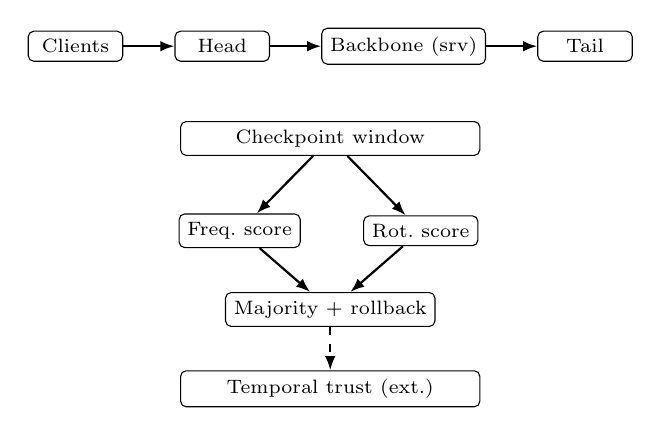
\begin{tikzpicture}[
      font=\scriptsize,
      box/.style={draw, rounded corners=2pt, align=center, inner sep=3pt, minimum width=1.2cm},
      arr/.style={-{Latex[length=1.8mm]}, thick},
    ]
    \node[box] (c) {Clients};
    \node[box, right=0.65cm of c] (h) {Head};
    \node[box, right=0.65cm of h] (b) {Backbone (srv)};
    \node[box, right=0.65cm of b] (t) {Tail};
    \draw[arr] (c) -- (h);
    \draw[arr] (h) -- (b);
    \draw[arr] (b) -- (t);

\node[box, below=0.95cm of $(c)!0.5!(t)$, minimum width=3.8cm] (win) {Checkpoint window};

\node[box] (dct) at ($(win.south)+(-1.15cm,-0.95cm)$) {Freq.\ score};
\node[box] (rot) at ($(win.south)+( 1.15cm,-0.95cm)$) {Rot.\ score};

\node[box] (maj) at ($(win.south)+(0cm,-1.95cm)$) {Majority + rollback};

\draw[arr] (win) -- (dct);
\draw[arr] (win) -- (rot);
\draw[arr] (dct) -- (maj);
\draw[arr] (rot) -- (maj);

    \node[box, below=0.55cm of maj, minimum width=3.8cm] (trust) {Temporal trust (ext.)};
    \draw[arr, dashed] (maj) -- (trust);
  \end{tikzpicture}%
  }}
  \caption{Summary figure of the reproduced SafeSplit pipeline and the implemented temporal trust extension. Activations flow through head, backbone, and tail; SafeSplit scores checkpoints in a window and rolls back when needed; the extension updates per client trust after repeated suspicious behavior.}
  \label{fig:overview}
\end{figure}

\begin{figure}[t]
  \centering
  \includegraphics[width=\linewidth]{figures/checkpoint-scoring.png}
  \caption{Checkpoint scoring example over one active window. The highest DCT score appears at checkpoint 1, while checkpoints 2 and 3 are most consistent with the benign majority. Checkpoint 4 is not the lowest score, but it remains inside the benign set and is therefore selected as the latest safe checkpoint. This illustrates why SafeSplit keeps the latest benign state rather than the absolute minimum score.}
  \label{fig:checkpoint_scoring}
\end{figure}

Figure~\ref{fig:checkpoint_scoring} is helpful for interpreting the implementation. The checkpoint with the strongest anomaly signal is not automatically the only one rejected by the defense. Instead, the defense looks for overlap between the benign majority under both views and then keeps the most recent checkpoint that still belongs to that overlap. This is a subtle but important point: SafeSplit is designed to preserve forward progress when possible, not simply to jump back to the globally most central checkpoint.

\section{Reproducing results}
\label{sec:results}

\subsection{Experimental setup and protocol}
\label{sec:setup}

Experiments use CIFAR-10 \cite{krizhevsky2009cifar} with a main label style partition that mixes independent and identically distributed draws according to a configurable IID rate $\rho$: each client's label distribution blends uniform draws with draws biased toward a main label, controlled by $\rho$ \cite{safesplit2025}. Models use a ResNet-18 backbone under the project \texttt{paper} preset. Reported metrics are main task accuracy on clean test data (MA) and backdoor accuracy on triggered test data (BA); lower BA indicates stronger suppression of the backdoor behavior.

The reported configuration is the one actually used for the final tables and plots. It consists of:
\begin{itemize}
    \item ResNet-18 architecture
    \item 10 clients, of which 2 are malicious
    \item 5 communication rounds
    \item 1 local epoch per client session
    \item batch size 128 and evaluation batch size 256
    \item default IID rate $\rho = 0.8$
    \item SafeSplit window size equal to the number of clients
    \item seed 42 for the reported comparison runs
\end{itemize}

These settings are important because they define the exact scope of the reproduction. The project does not claim to reproduce every experiment in the original paper. Instead, it focuses on the main CIFAR-10 comparisons that are most informative for the course objectives: Table II style defense comparison, Table III style IID sweep, reduced baselines, and the implemented trust extension under slow poisoning.

Table~\ref{tab:hyper} lists fixed hyperparameters for the \texttt{paper} preset as implemented in \texttt{config.py}. The notebook selects a reporting seed from a small candidate list so that SafeSplit semantic rows remain informative under stochastic training; all tables in this report use seed $42$. Implementations rely on PyTorch \cite{paszke2019pytorch}.

\begin{table}[t]
  \caption{Paper preset hyperparameters (see \texttt{config.py}).}
  \label{tab:hyper}
  \begin{center}
    \begin{small}
      \begin{tabular}{lr}
        \toprule
        Setting & Value \\
        \midrule
        Clients / malicious & $10$ / $2$ \\
        Communication rounds & $5$ \\
        Local epochs per session & $1$ \\
        Batch size / eval batch & $128$ / $256$ \\
        Learning rate & $10^{-3}$ \\
        Default IID rate $\rho$ & $0.8$ \\
        SafeSplit window size & $10$ (matches clients) \\
        \bottomrule
      \end{tabular}
    \end{small}
  \end{center}
\end{table}

\subsection{Threat model and attack schedules}
\label{sec:threat}

Malicious clients inject backdoors via local datasets. The \emph{pixel} attack stamps a small trigger and relabels toward a target class; the \emph{semantic} attack maps a source class to a target class without a patch. For temporal trust, \emph{slow poisoning} ramps the poisoned data rate from $0.05$ to $0.50$ across rounds (\texttt{ScheduledPoisonedDataset}, \texttt{attack\_schedule}). Primary experiments use a fixed poison rate $0.50$ unless slow poisoning is enabled.

This distinction matters. The standard reproduction experiments test whether SafeSplit can suppress strong attacks under a fixed poisoning rate. The extension experiments test whether the defense can remain informative when a malicious client starts gently and becomes more aggressive over time. In other words, the extension evaluates a more temporally subtle threat model.

\subsection{Defense comparison}
\label{sec:table2}

Table~\ref{tab:table2} lists pixel and semantic attacks with and without SafeSplit at IID rate $0.8$. Figure~\ref{fig:table2chart} shows the same quantities as a bar chart exported from the notebook suite. Without defense, both attacks reach nearly perfect BA while MA stays near random to moderate on this short horizon setup. SafeSplit removes the semantic backdoor entirely (BA $0\%$) and reduces pixel BA from $99.9\%$ to $7.5\%$, at the cost of lower MA because aggressive rollback and filtering affect the converged clean accuracy.

\begin{table}[t]
  \caption{Defense comparison aligned with Table II style experiments (IID rate $0.8$, paper preset, reporting seed $42$).}
  \label{tab:table2}
  \begin{center}
    \begin{small}
      \begin{tabular}{llrr}
        \toprule
        Attack & Defense & MA (\%) & BA (\%) \\
        \midrule
        pixel & none & 51.96 & 99.90 \\
        pixel & SafeSplit & 45.28 & 7.54 \\
        semantic & none & 53.37 & 100.00 \\
        semantic & SafeSplit & 44.89 & 0.00 \\
        \bottomrule
      \end{tabular}
    \end{small}
  \end{center}
\end{table}

\begin{figure}[t]
  \centering
  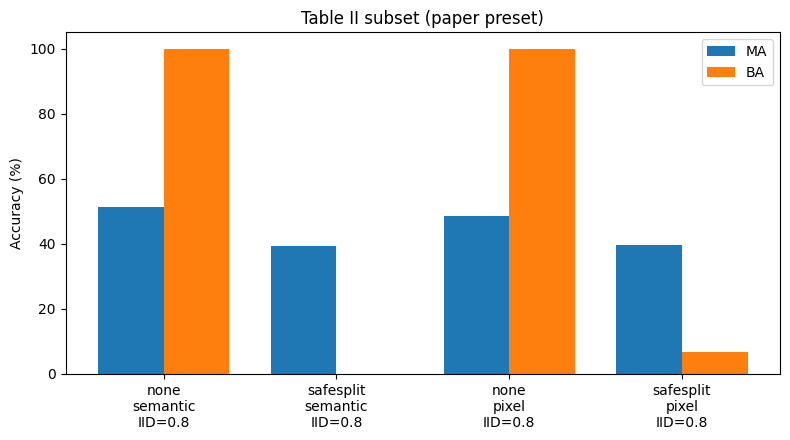
\includegraphics[width=\linewidth]{figures/table-ii-chart.png}
  \caption{Bar chart for Table~\ref{tab:table2}: MA and BA across attack and defense settings.}
  \label{fig:table2chart}
\end{figure}

Compared with the original paper, our reproduction matches the main qualitative behavior: attacks are highly effective without defense, while SafeSplit sharply reduces BA and keeps MA usable. Exact numerical matching is not expected here because the project uses a simplified implementation and backdoor experiments are sensitive to trigger construction, client partitioning, random seed, and training details. In particular, our semantic attack is harsher without defense and our pixel SafeSplit run leaves more residual BA than the paper, but the overall defense trend is the same.

This comparison is important for the course evaluation criteria. The goal of the reproduction is not to claim that every number is identical to the paper, but to show that the same experimental logic produces the same broad conclusion. In that sense, Table~\ref{tab:table2} is successful: the undefended attack is highly effective, SafeSplit sharply reduces the attack, and the tradeoff is visible in MA. More specifically, the semantic case is the cleanest qualitative match: no defense drives BA to its maximum, while SafeSplit drives BA to zero. The pixel case is slightly weaker numerically, because residual BA remains, but the direction of the effect is still consistent with the paper.

\subsection{Semantic attack across IID rates}
\label{sec:table3}

Table~\ref{tab:table3} compares none versus SafeSplit for three IID rates. Figure~\ref{fig:table3chart} plots MA and BA across those rates. The undefended semantic attack keeps BA at $100\%$ for every $\rho$; SafeSplit holds BA at $0\%$ across the sweep. As $\rho$ increases, MA rises for both settings because clients see more balanced label mixtures; SafeSplit consistently trades some MA relative to no defense for complete backdoor removal in these runs.

\begin{table}[t]
  \caption{Semantic attack across IID rates (paper preset, reporting seed $42$). N: no defense; SS: SafeSplit.}
  \label{tab:table3}
  \begin{center}
    \adjustbox{max width=\linewidth}{
    \begin{small}
      \begin{tabular}{lrrrr}
        \toprule
        $\rho$ & N-MA & N-BA & SS-MA & SS-BA \\
        \midrule
        0.6 & 49.81 & 100.00 & 41.64 & 0.00 \\
        0.8 & 52.70 & 100.00 & 45.40 & 0.00 \\
        1.0 & 55.70 & 100.00 & 46.34 & 0.00 \\
        \bottomrule
      \end{tabular}
    \end{small}
    }
  \end{center}
\end{table}

\begin{figure}[t]
  \centering
  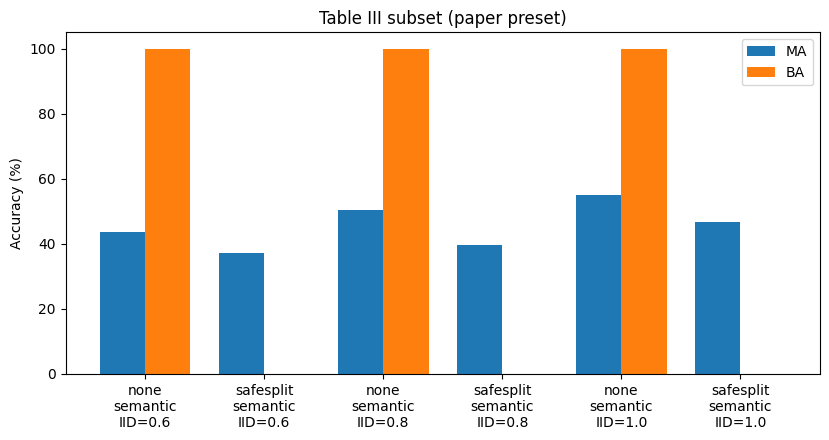
\includegraphics[width=\linewidth]{figures/table-iii-chart.png}
  \caption{IID sweep for the semantic attack: MA and BA for none and SafeSplit.}
  \label{fig:table3chart}
\end{figure}

This section shows that the reproduction is not tied to only one easiest data distribution. As the data become more IID, MA improves for both defended and undefended runs. That is intuitive because clients see more balanced data. At the same time, SafeSplit keeps BA at zero across the whole sweep. This makes the result stronger than a single point estimate: the defense remains effective even when the client label distributions change.

A useful way to interpret Table~\ref{tab:table3} is that client heterogeneity mainly affects \emph{clean learning difficulty}, while SafeSplit still retains its qualitative backdoor suppression behavior. This is one of the clearest places where the reproduction supports the original paper's message. It also makes the report stronger formally, because it shows that the reproduction is not limited to one isolated configuration but examines the defense under varying client data distributions.

\subsection{Reduced baselines}
\label{sec:baselines}

The codebase includes simplified baselines in \texttt{defense/baselines.py}. \emph{Differential privacy} clips the $\ell_2$ norm of the backbone update vector, scales updates, and adds Gaussian noise to backbone weights after each selection. \emph{KRUM style} defense compares Euclidean distances between flattened update vectors in a window and returns the checkpoint whose summed distance to its nearest peers is minimal.

Table~\ref{tab:baseline} summarizes these baselines together with SafeSplit at IID rate $0.6$ under the semantic attack. Figure~\ref{fig:baselinechart} visualizes MA and BA. In this configuration, the DP baseline drives BA to zero but collapses MA ($10\%$), illustrating an aggressive accuracy tradeoff. KRUM style defense also removes the backdoor but attains lower MA than SafeSplit ($37.4\%$ vs.\ $41.6\%$).

\begin{table}[t]
  \caption{Reduced baseline panel at IID rate $0.6$ (semantic attack, paper preset).}
  \label{tab:baseline}
  \begin{center}
    \begin{small}
      \begin{tabular}{lrr}
        \toprule
        Defense & MA (\%) & BA (\%) \\
        \midrule
        none & 49.81 & 100.00 \\
        differential privacy & 10.00 & 0.00 \\
        KRUM style & 37.43 & 0.00 \\
        SafeSplit & 41.64 & 0.00 \\
        \bottomrule
      \end{tabular}
    \end{small}
  \end{center}
\end{table}

\begin{figure}[t]
  \centering
  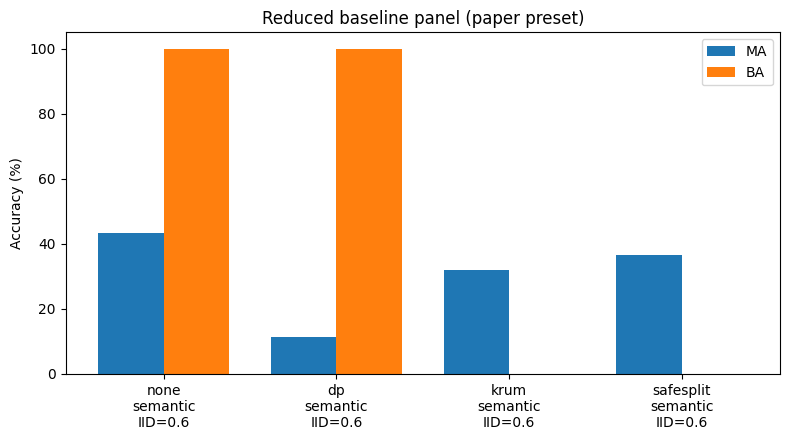
\includegraphics[width=\linewidth]{figures/baseline-chart.png}
  \caption{Baseline comparison at IID rate $0.6$: MA and BA.}
  \label{fig:baselinechart}
\end{figure}

This baseline panel is helpful because it shows that simply achieving BA $=0$ is not enough. The DP baseline does remove the backdoor in this run, but its clean accuracy collapses. KRUM style defense also reaches BA $=0$, yet it keeps less useful clean performance than SafeSplit. Therefore, SafeSplit is strongest here not because it is the only successful defense, but because it gives the best balance between preserving the main task and suppressing the backdoor.

This comparison is also valuable for the final report because the course criteria emphasize both correctness of reproduction and meaningful performance analysis. The baseline panel demonstrates that our evaluation is not limited to a single defense versus no defense comparison. Instead, it places SafeSplit inside a smaller but still informative comparison set, which strengthens the claim that its behavior in our reproduction is meaningful rather than accidental.

\subsection{Limitations of the reproduction}
\label{sec:limits}

The report uses a single reporting seed after candidate search, and MA can shift across seeds while the broad ranking often persists. Training uses five rounds on CIFAR-10. These results should therefore be read as a focused reproduction that captures the paper's qualitative behavior rather than a claim of exact numerical replication.

Another limitation is that the reproduction deliberately focuses on CIFAR-10 and a reduced subset of the paper's experimental scope. This is appropriate for a course project, but it means that the conclusions are strongest for the chosen setting rather than for every dataset and architecture used in the original paper.

\section{Proposed improvement}
\label{sec:extension}

\subsection{Limitation addressed}

The original SafeSplit mechanism tracks checkpoint history inside a bounded window, but it does not explicitly maintain persistent client reliability across rounds. An attacker who slowly increases poisoning can therefore produce updates that remain near the benign boundary for several sessions. Server side decisions that look only at the current window may react later than desired even when suspicious behavior repeats over time.

This limitation is important because the defense may be correct locally but still forget useful historical context. If the same client repeatedly behaves slightly suspiciously, a purely window based rule may treat each event as isolated. The temporal trust extension addresses exactly that gap.

\subsection{Temporal trust score}

The extension maintains a scalar trust value per client in $[0,1]$. In the current implementation, the client set remains fixed during training. After each session, the implementation reads normalized suspiciousness from SafeSplit and applies a reward when suspiciousness lies below a soft threshold and the session falls in the benign majority; otherwise it applies a penalty proportional to suspiciousness. When trust falls below a fixed threshold, the defense records a low trust flag and can bias rollback toward checkpoints from higher trust clients.

In plain words, trust increases slightly after benign low suspiciousness behavior, decreases after suspicious behavior, and a client becomes low trust once its score falls below the low trust threshold. Reported runs use initial trust $1.0$, reward $0.02$, penalty scale $0.10$, soft threshold $0.60$, and low trust threshold $0.70$ from \texttt{config.py}.

Let $s$ denote normalized suspiciousness and let $\mathcal{B}$ be the benign majority set from SafeSplit. With reward $r$, penalty $\lambda$, soft threshold $\tau$, and trust threshold $\theta$, the update is
\[
\begin{array}{l}
\mathrm{trust} \leftarrow \min\bigl(1,\, \mathrm{trust}+r\bigr)
\quad \text{if } s < \tau \text{ and session} \in \mathcal{B}, \\[2pt]
\mathrm{trust} \leftarrow \max\bigl(0,\, \mathrm{trust}-\lambda s\bigr)
\quad \text{otherwise,} \\[2pt]
\text{low trust flag} \Leftarrow (\mathrm{trust} \le \theta).
\end{array}
\]

There is a tradeoff in these thresholds. A stricter threshold can flag suspicious clients earlier and may help slow poisoning detection, but it can also penalize benign sessions and reduce MA. A looser threshold is safer for MA but may delay trust based separation. The threshold is therefore not only a detection parameter but also an MA and BA tradeoff parameter.

\subsection{Slow poisoning schedule}

The attack schedule increases the poisoned data rate from $0.05$ at the start of training to $0.50$ at the end across the configured number of rounds, using a dataset wrapper that updates the active poisoning rate between rounds.

This experiment is the most natural place to test temporal trust. If the poisoning rate starts high immediately, SafeSplit often already reacts strongly. But in slow poisoning, the attacker tries to remain close to benign behavior at first. This makes repeated client level tracking more valuable, because the goal is not only to reject one dramatic update, but to accumulate evidence over time.

\subsection{Extension results}

Table~\ref{tab:trust} lists slow poisoning runs under IID rate $0.8$. Both SafeSplit and SafeSplit with temporal trust achieve BA $0.00$, while training without defense reaches BA $100.00$. Mean trust after training is lower for malicious clients than for benign clients when temporal trust is enabled, and the run logs three low trust flags. Clean accuracy remains similar between SafeSplit and SafeSplit with trust ($39.08\%$ vs.\ $39.51\%$), suggesting the trust layer adds client level temporal information without undoing rollback gains on this schedule.

\begin{table}[t]
  \caption{Slow poisoning experiment (IID rate $0.8$, attack schedule slow). Mal.\ / Ben.\ trust: mean trust for malicious vs.\ benign clients.}
  \label{tab:trust}
  \begin{center}
    \adjustbox{max width=\linewidth}{
    \begin{small}
      \begin{tabular}{lrrrrr}
        \toprule
        Defense & MA (\%) & BA (\%) & Mal.\ trust & Ben.\ trust & Flags \\
        \midrule
        none & 51.34 & 100.00 & -- & -- & 0 \\
        SafeSplit & 39.08 & 0.00 & -- & -- & 0 \\
        SafeSplit + trust & 39.51 & 0.00 & 0.63 & 0.82 & 3 \\
        \bottomrule
      \end{tabular}
    \end{small}
    }
  \end{center}
\end{table}

The extension therefore should not be read as a large BA improvement over SafeSplit in this reported run, because SafeSplit already reaches BA $=0.00$. Instead, the improvement is that it preserves SafeSplit's BA suppression while adding temporal client tracking, low trust flags, and a small MA gain under slow poisoning.

This is the correct way to interpret the result academically. The improvement is not ``SafeSplit plus trust always beats SafeSplit on BA.'' The improvement is that the trust layer provides extra client level information and exposes repeated mild malicious behavior without weakening the original defense. That makes the extension meaningful even when BA is already minimized by the base method.

The trust gap itself is also meaningful. Malicious clients finish with lower average trust than benign clients, and low trust flags appear only when the temporal score accumulates enough evidence. This is exactly the intended behavior of the extension. It does not replace SafeSplit's checkpoint analysis, but it adds a second level of interpretation across rounds. From a systems perspective, this is valuable because it gives the server a persistent client level signal instead of only a one window checkpoint decision.

\section{Conclusions and future directions}
\label{sec:conclusion}

The reproduction aligns qualitatively with SafeSplit: semantic and pixel attacks succeed without defense, while SafeSplit suppresses semantic backdoors across IID settings and reduces pixel backdoors substantially in this codebase \cite{safesplit2025}. The temporal trust extension complements checkpoint analysis by accumulating evidence across rounds and separating average trust for malicious and benign clients under slow poisoning without reversing SafeSplit's backdoor suppression.

From a course project perspective, the two objectives are both satisfied. First, the reproduction captures the main experimental behavior of the paper on the chosen CIFAR-10 scope. Second, the proposed improvement is implemented and evaluated rather than only suggested conceptually. The extension does not claim a dramatic BA improvement beyond SafeSplit, but it does provide a concrete improvement in temporal malicious client tracking.

Future work includes scaling to larger models and datasets, adaptive thresholds that depend on round index or window length, and experiments where clients can join or leave so trust states must handle membership change.

\section*{Code availability}
\label{sec:code}

All software, the notebook \texttt{SafeSplit\_walkthrough.ipynb}, command line runners \texttt{main.py} and \texttt{run\_experiments.py}, and generated figures under \texttt{assets/readme/} are available at \url{https://github.com/MateoLopez00/SafeSplit_Distributed_DL}.

\bibliography{references}
\bibliographystyle{icml2025}

\end{document}